\documentclass[12pt]{article}
\usepackage[margin=1in]{geometry}
\usepackage{graphicx}
\usepackage{booktabs}
\usepackage{amsmath}
\usepackage{amssymb}
\usepackage{float}
\usepackage{caption}
\usepackage{setspace}
\usepackage[most]{tcolorbox}
\captionsetup{font=small, labelfont=bf, skip=6pt}
\onehalfspacing

\newtcolorbox{explain}{%
  colback=black!3,
  colframe=black!25,
  boxrule=0.5pt,
  arc=1pt,
  left=8pt,
  right=8pt,
  top=5pt,
  bottom=5pt,
  before skip=6pt,
  after skip=12pt,
  fontupper=\normalsize
}

\title{Feature Engineering\\[0.2em]
\large Bitcoin realized volatility}
\author{Volatility forecasting project}
\date{29 September 2026}

\begin{document}
\maketitle

\noindent
This note locks the target and which inputs each model family uses.
Only complete UTC days enter the panel (24 valid hourly log returns).
Everything at date \(t\) is known by the close of day \(t\).
RSI, Bollinger bands, rolling skewness/kurtosis, and price MAs stay in the EDA report only.

\section{Target}
\[
y_t=\log\mathrm{RV}_{t+1},
\qquad
\mathrm{RV}_{t}=\sqrt{\sum_{i\in t} r_{t,i}^2}.
\]
\begin{figure}[H]
\centering
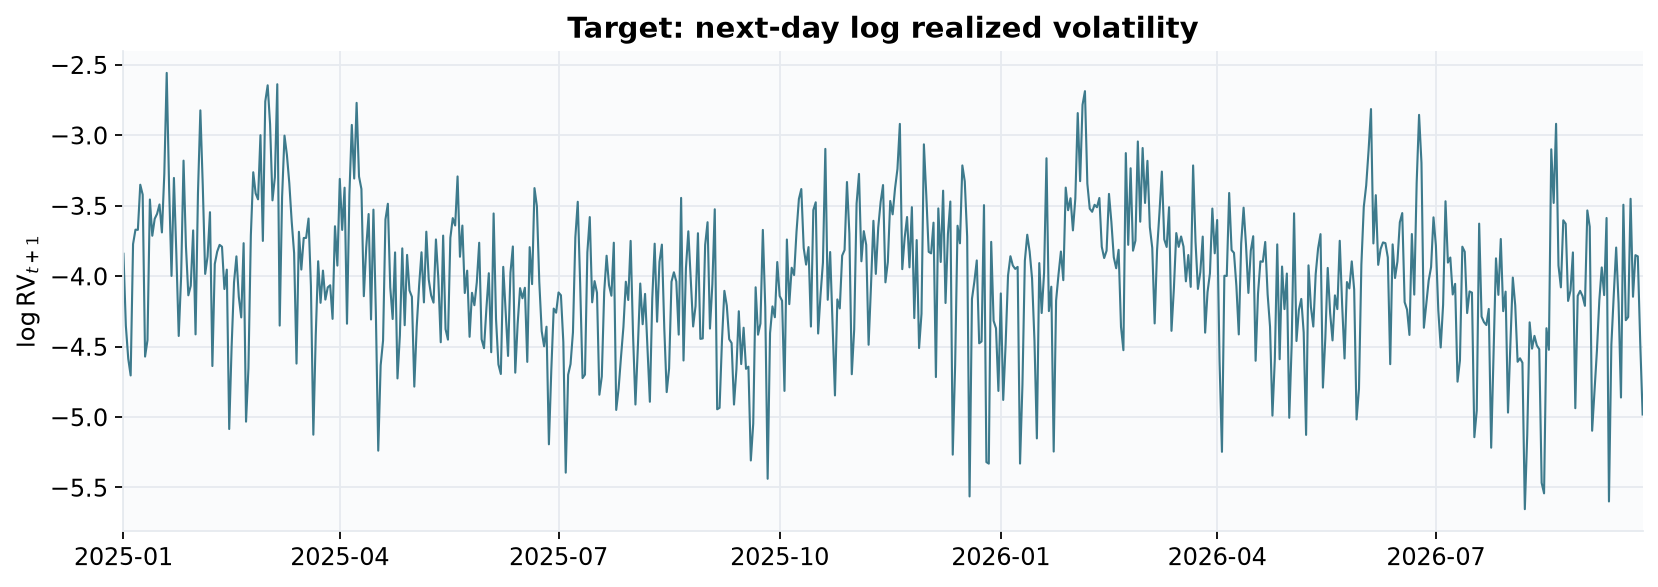
\includegraphics[width=\textwidth]{figures/target_y.png}
\caption{Target series \(y_t=\log\mathrm{RV}_{t+1}\) (display window from 2025).}
\end{figure}
\begin{explain}
The project forecasts \(\log\mathrm{RV}_{t+1}\) (not price). Raw RV is right-skewed; \(\log\mathrm{RV}\) is nearly symmetric. The last day has no \(y_t\) because tomorrow's RV is unobserved.
\end{explain}

\section{Sample and leakage rules}
\begin{table}[H]
\centering
\begin{tabular}{lr}
\toprule
Complete UTC days & 3{,}298 \\
Model-ready rows & 3{,}268 \\
Dropped (warmup / no \(y\)) & 30 \\
HAR week window & 7 days \\
HAR month window & 22 days \\
Volume \(z\) window & 30 days \\
\bottomrule
\end{tabular}
\caption{Panel coverage after requiring a full lookback and a next-day target.}
\end{table}
\begin{explain}
Warmup drops come from the 30-day volume \(z\) and HAR windows; one final row is dropped because \(y_t\) needs day \(t+1\). No future information enters features at \(t\).
\end{explain}

\section{Who uses what}
\begin{table}[H]
\centering
\begin{tabular}{lll}
\toprule
Model & Input & Forecast \\
\midrule
Naive & \(\log\mathrm{RV}_t\) & \(\widehat y_t=\log\mathrm{RV}_t\) \\
HAR & \(\log\mathrm{RV}^{(d)},\log\mathrm{RV}^{(w)},\log\mathrm{RV}^{(m)}\) & \(\widehat{\log\mathrm{RV}}_{t+1}\) \\
ARIMA & \(\log\mathrm{RV}\) series (orders on that series) & \(\widehat{\log\mathrm{RV}}_{t+1}\) \\
GARCH-family & daily return series \(R_t\) & \(\hat\sigma_{t+1}\), scored vs \(\mathrm{RV}_{t+1}\) \\
LSTM & length-\(L\) window of \(\log\mathrm{RV}\) (+ optional auxiliaries) & \(\widehat{\log\mathrm{RV}}_{t+1}\) \\
\bottomrule
\end{tabular}
\caption{Model-specific inputs. Models do not all consume the same wide feature row.}
\end{table}
\begin{explain}
HAR and ARIMA are realized-vol-on-vol. GARCH filters returns and produces conditional volatility \(\hat\sigma_{t+1}\), which is compared to realized \(\mathrm{RV}_{t+1}\) as forecast vs outcome---not renamed RV. LSTM sees a \emph{sequence} of past \(\log\mathrm{RV}\) (e.g.\ last 22 days), not a single static row of three HAR averages.
\end{explain}

\section{HAR-style log-RV features}
\[
\log\mathrm{RV}^{(d)}_t=\log\mathrm{RV}_t,
\quad
\log\mathrm{RV}^{(w)}_t=\frac1{7}\sum_{i=0}^{6}\log\mathrm{RV}_{t-i},
\quad
\log\mathrm{RV}^{(m)}_t=\frac1{22}\sum_{i=0}^{21}\log\mathrm{RV}_{t-i}.
\]
\begin{figure}[H]
\centering
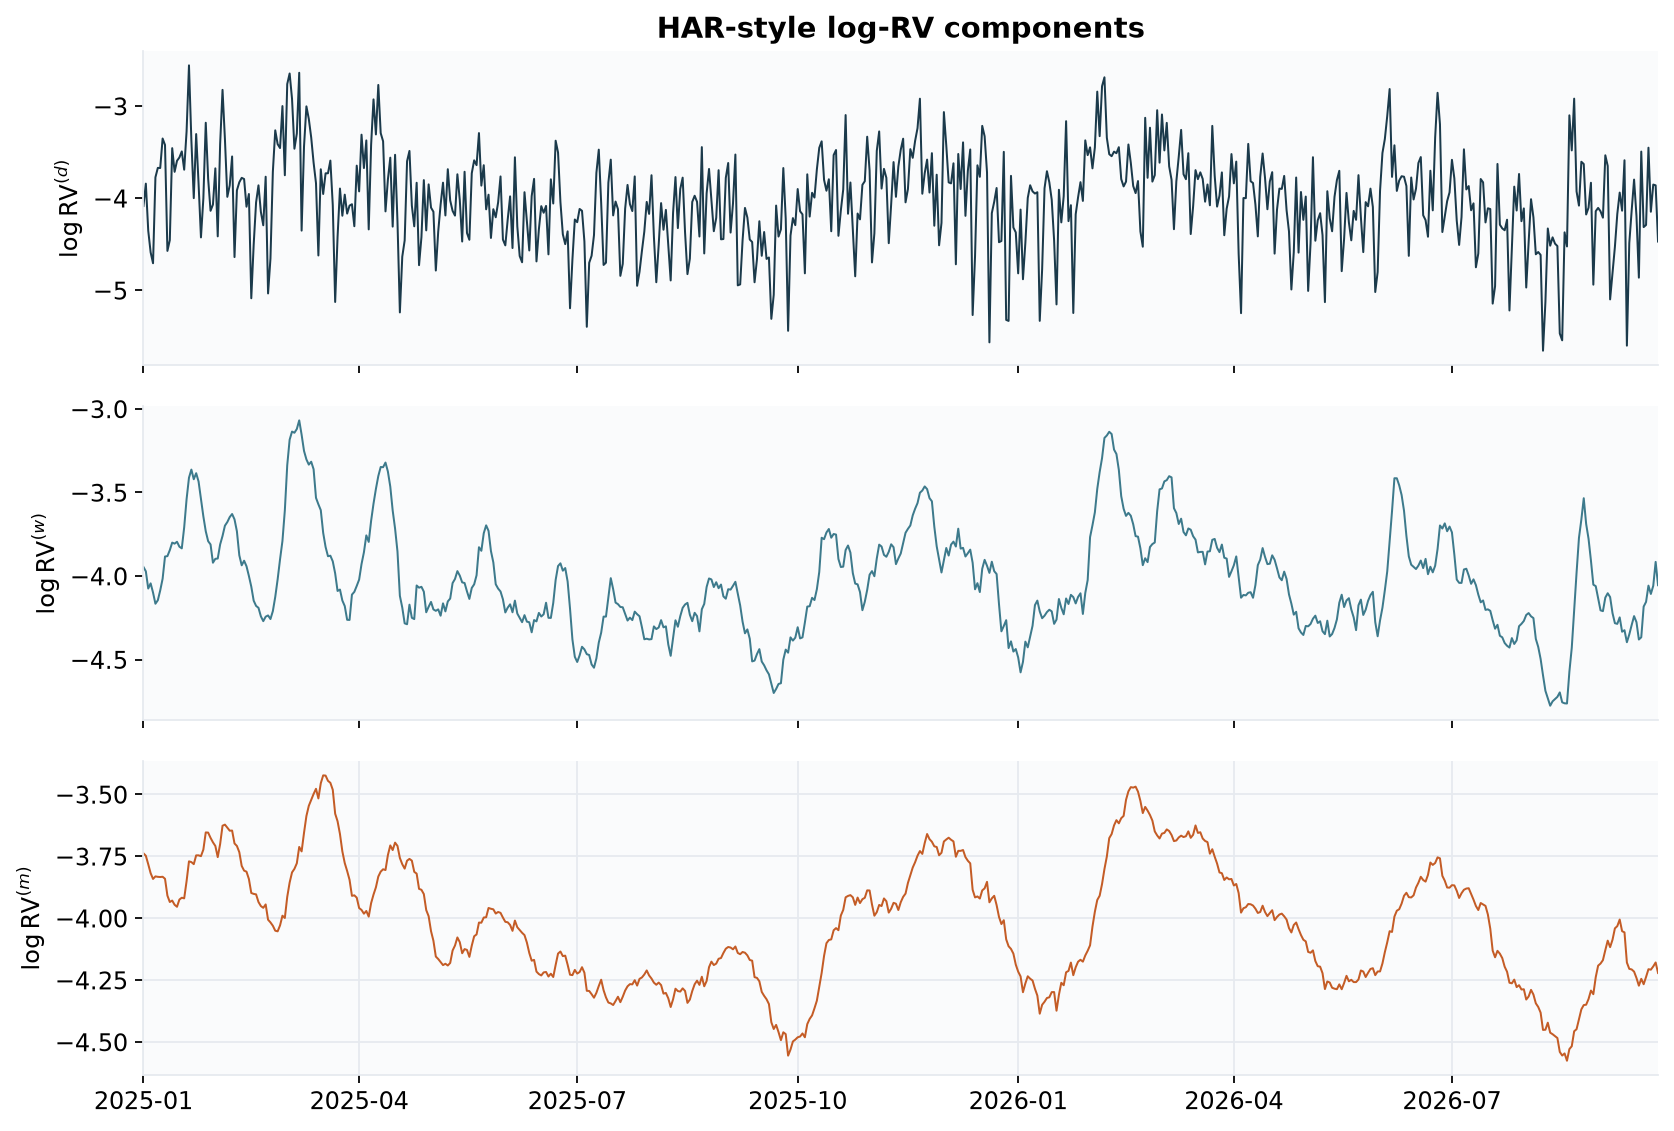
\includegraphics[width=\textwidth]{figures/har_components.png}
\caption{Daily, weekly, and monthly log-RV components.}
\end{figure}
\begin{explain}
Crypto trades every calendar day, so the week average uses 7 days (not a 5-day equity week). The month term uses 22 days. These three terms are the HAR regressors.
\end{explain}

\section{Returns (GARCH series; optional LSTM auxiliary)}
\[
R_t=\sum_{i\in t} r_{t,i},
\qquad
R_t^2.
\]
\begin{figure}[H]
\centering
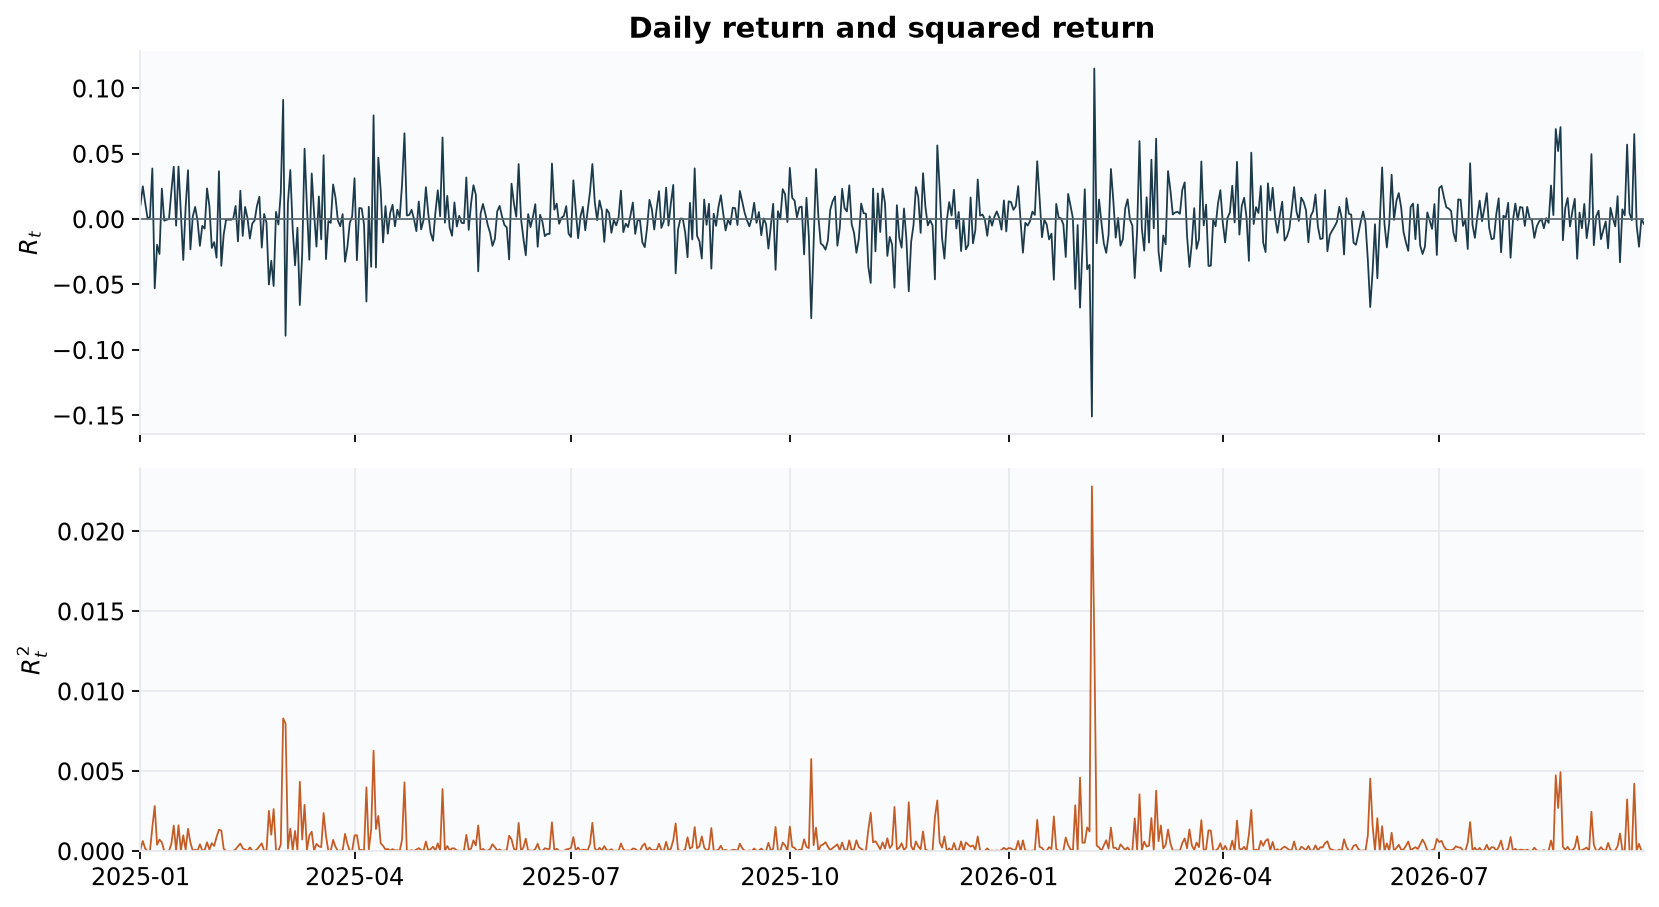
\includegraphics[width=\textwidth]{figures/return_features.png}
\caption{Daily log return and squared return.}
\end{figure}
\begin{explain}
\(R_t\) is the input \emph{series} for GARCH-family models---not a HAR covariate. \(R_t^2\) is an optional LSTM channel (shock size). Raw \(R_t\) is a weak linear predictor of \(y_t\) and is not a core LSTM feature.
\end{explain}

\section{Volume \(z\)-score (optional LSTM auxiliary)}
\[
Z^{(30)}_t=\frac{V_t-\mu^{(30)}_t}{\sigma^{(30)}_t}.
\]
\begin{figure}[H]
\centering
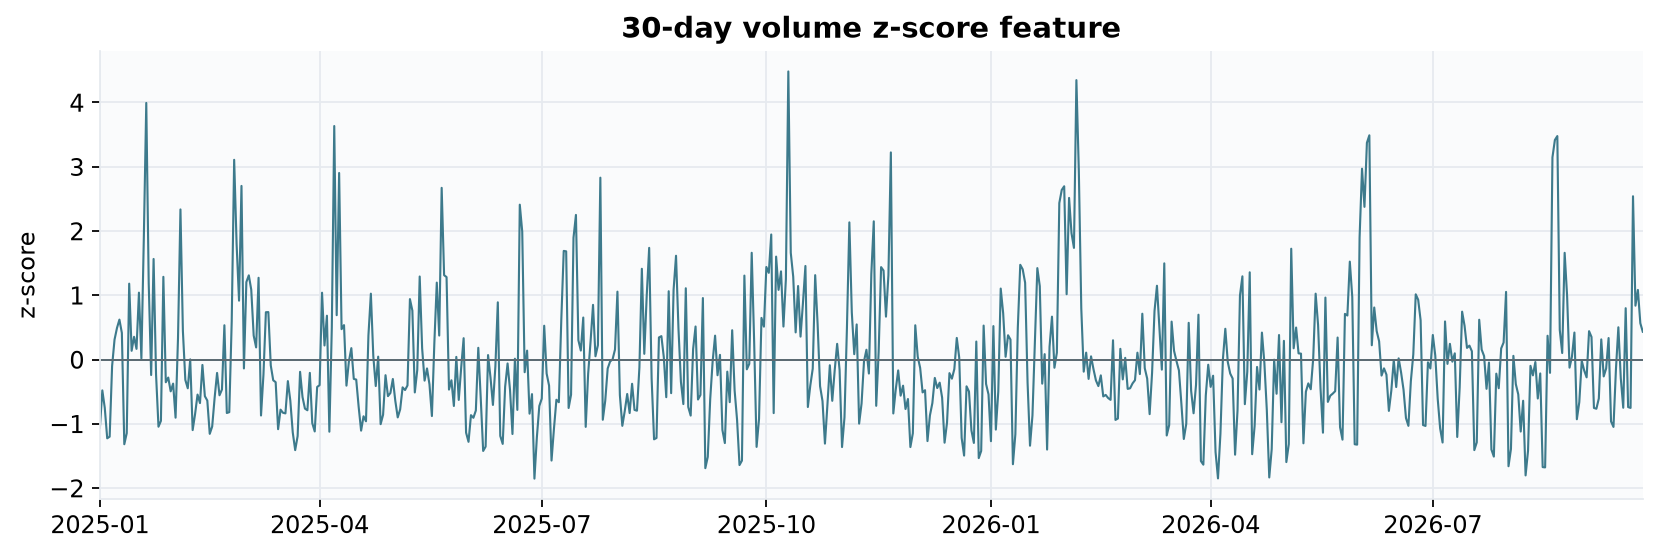
\includegraphics[width=\textwidth]{figures/volume_z_feature.png}
\caption{30-day volume \(z\)-score.}
\end{figure}
\begin{explain}
Activity shocks often accompany volatility bursts. Kept as an optional extra channel in the LSTM window alongside \(\log\mathrm{RV}\). Not used by HAR, ARIMA, or GARCH.
\end{explain}

\section{Feature–target association}
\begin{figure}[H]
\centering
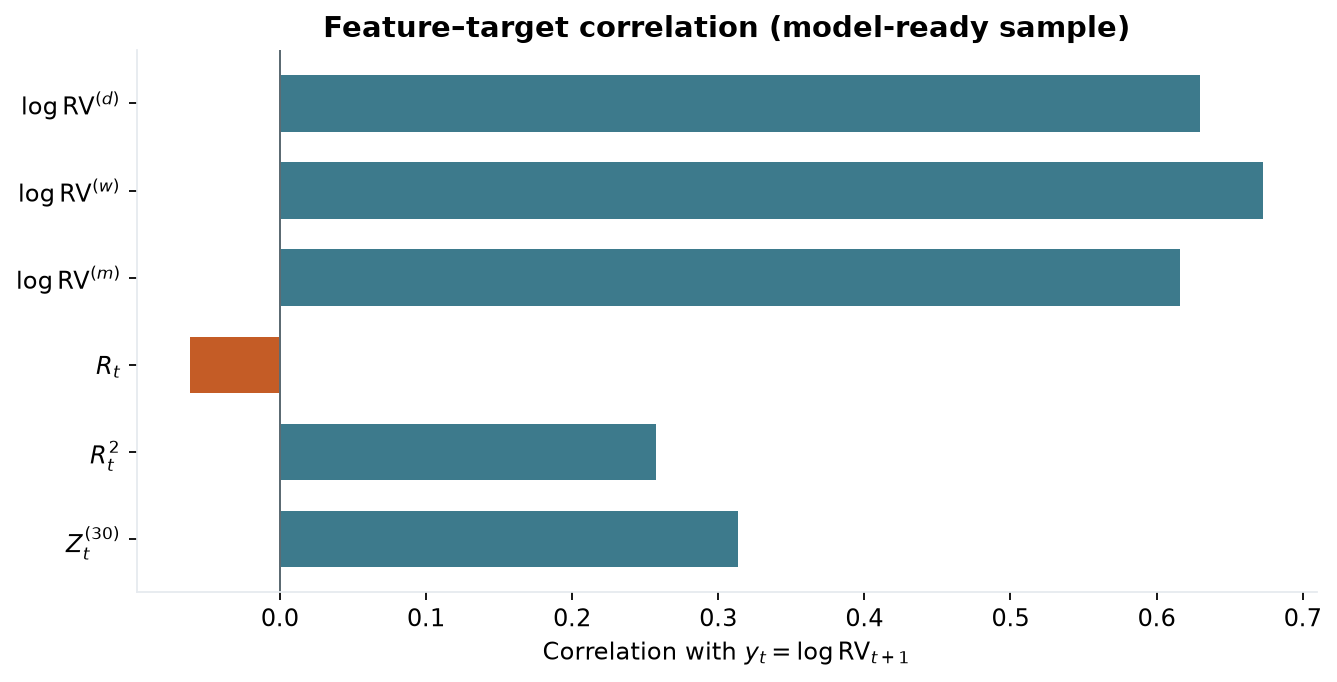
\includegraphics[width=0.92\textwidth]{figures/corr_with_y.png}
\caption{Pearson correlation of panel columns with \(y_t\).}
\end{figure}
\begin{figure}[H]
\centering
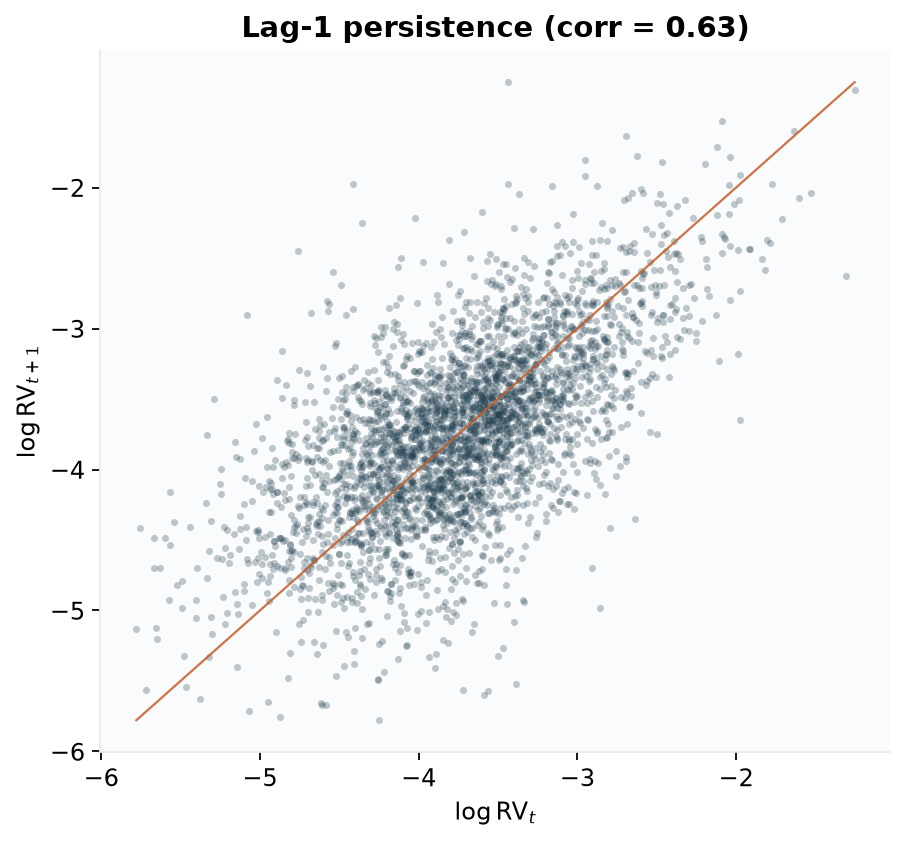
\includegraphics[width=0.72\textwidth]{figures/lag1_scatter.png}
\caption{\(\log\mathrm{RV}_t\) against \(\log\mathrm{RV}_{t+1}\).}
\end{figure}
\begin{explain}
HAR-style log-RV terms dominate (correlations about \(0.62\)--\(0.67\)). Volume \(z\) and \(R_t^2\) are moderate. Signed \(R_t\) is near zero---useful as GARCH's data process, not as a stand-alone predictor of next-day \(\log\mathrm{RV}\).
\end{explain}

\section{Collinearity among panel columns}
\begin{figure}[H]
\centering
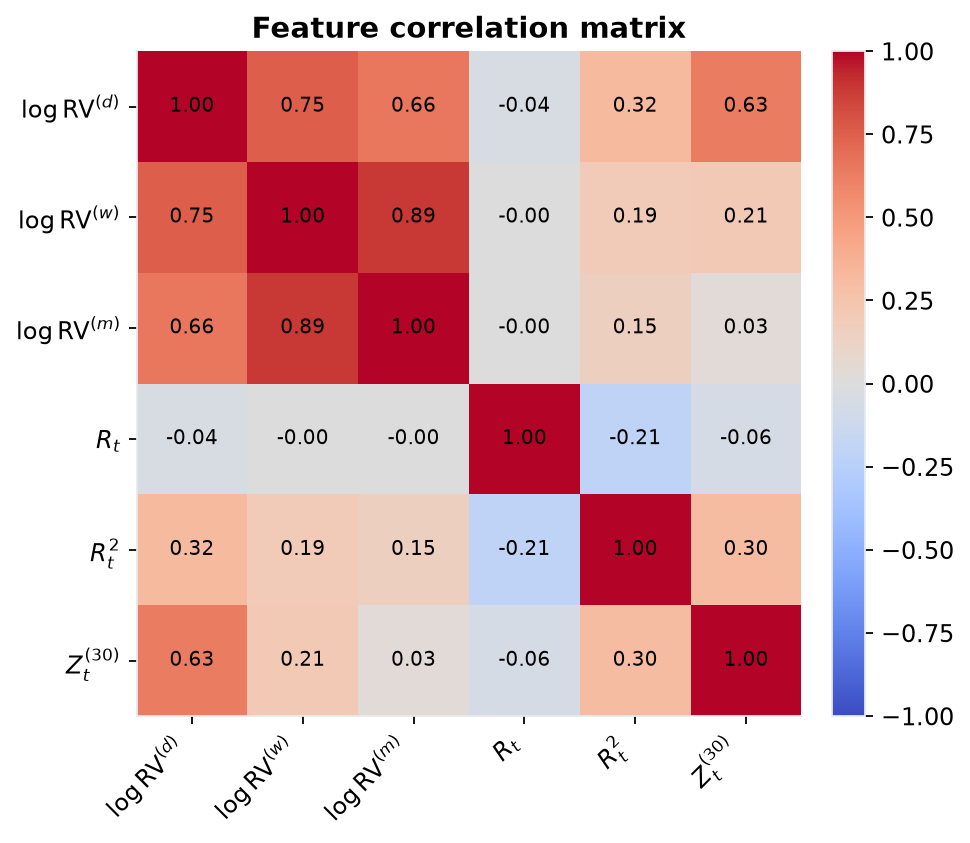
\includegraphics[width=0.78\textwidth]{figures/feature_corr.png}
\caption{Pairwise correlations (red $=$ strong positive, blue $=$ strong negative).}
\end{figure}
\begin{explain}
The large red block among \(\log\mathrm{RV}^{(d)}\), \(\log\mathrm{RV}^{(w)}\), and \(\log\mathrm{RV}^{(m)}\) is expected: the week and month terms are rolling averages of the same series, so they move together by construction (pairwise correlations about \(0.66\)--\(0.89\)). That is \emph{not} a signal to delete two HAR lags. HAR is designed that way; coefficients are read jointly as a multi-horizon decomposition, not as three independent effects. Signed \(R_t\) is almost uncorrelated with the HAR block. Volume \(z\) moves with daily \(\log\mathrm{RV}\) (about \(0.63\)) but much less with the month term---overlap, not a reason to drop the HAR structure.
\end{explain}

\section{Panel columns vs model inputs}
\begin{table}[H]
\centering
\begin{tabular}{llll}
\toprule
Column & Definition & HAR/ARIMA & GARCH / LSTM \\
\midrule
\texttt{log\_rv\_d/w/m} & HAR log-RV terms & HAR uses all three & LSTM uses lag window of \texttt{log\_rv} \\
\texttt{log\_rv} & daily \(\log\mathrm{RV}_t\) & ARIMA series & LSTM sequence core \\
\texttt{ret\_d} & \(R_t\) & --- & GARCH series \\
\texttt{ret\_d\_sq} & \(R_t^2\) & --- & optional LSTM channel \\
\texttt{volume\_z30} & volume \(z\) & --- & optional LSTM channel \\
\texttt{y} & \(\log\mathrm{RV}_{t+1}\) & target & target \\
\bottomrule
\end{tabular}
\caption{Same parquet panel; different models read different columns / shapes.}
\end{table}
\begin{explain}
File: \texttt{data/processed/btcusdt\_1d\_features.parquet}. Scaling for neural nets, if used, is fit on the training window only in the evaluation step.
\end{explain}

\section{Synthesis}
Target and leakage rules are locked.
HAR uses the three log-RV horizons; ARIMA uses the \(\log\mathrm{RV}\) series; GARCH uses returns and forecasts \(\hat\sigma_{t+1}\) against realized RV; LSTM uses a length-\(L\) window of \(\log\mathrm{RV}\), with \(R_t^2\) and volume \(z\) only as optional extras.
The red HAR correlations in the matrix are structural redundancy from nested averages, not a failed feature set.

\end{document}
